\section{Theorie}
\label{sec:Theorie}

In letzter Zeit ist es Wissenschaftlern gelungen, Gravitationswellen nachzuweisen.
Hierzu wurde ein Michelson-Interferometer benutzt, da es dazu geeignet ist, Wellenlängen, sowie deren absolute Änderung zu messen.
Zusätzlich können auch Brechungsindizes gemessen werden.
Das Michelson-Interferometer selbst stützt sich auf das Interferenzprinzip, auf welches im Folgenden weiter eingegangen wird.\\
Im allgemeinen kann Licht als elektromagnetische Welle der Form
\begin{equation}
  \vec{E}(x,t) = \vec{E_0}\exp{(i(\vec{k}\vec{x}-\omega t -\delta))}, \label{eqn:1}
\end{equation}
mit Ort $\vec{x}$ und Zeit $t$, sowie Wellenvektor $\vec{k}$, Frequenz $\omega$ und Phasenkonstante $\delta$, angenommen werden, wobei sie sich nur in ihrer Intensität
\begin{equation}
  I = const |\vec{E}|²
\end{equation}
messbar macht.
Da diese elektromagnetischen Wellen den Maxwell-Gleichungen unterliegen, gilt die lineare Superposition, wodurch sich zwei Wellen einfach addieren lassen.
Aus Gründen der Messbarkeit muss hier jedoch auf ein zeitliches Mittel zurückgegriffen werden, wodurch sich für die gesamte Intensität $I_{\text{ges}}$ der Ausdruck
\begin{equation}
  I_{\text{ges}} = \frac{const}{t_2-t_1} \int_{t_1}^{t_2} (|\vec{E_1}+\vec{E_2}|)²(x,t) dt
\end{equation}
ergibt. Dabei muss darauf geachtet werden, dass die Periodendauer $T = 2\pi/\omega$ groß gegenüber der Länge des Messintervalls ist.
Somit ergibt sich für zwei Lichtwellen der Form \ref{eqn:1}, welche sich nur in ihrer Phase unterscheiden,
\begin{equation}
  I_{\text{ges}} = const \cdot 2\vec{E_0}(1+\cos{\delta_2-\delta_1}).
\end{equation}
Hierbei spiegelt der Cosinus den Interferenzterm wieder.
Erkennbar ist, dass, wenn der Phasenunterschied $(\delta_2-\delta_1)$ ungerade Vielfache von $\pi$ beträgt, es zur Auslöschung der beobachtbaren Intensität führt.
Dies wird als destruktive Interferenz bezeichnet.
Ein Kernkriterium, unter dem Interferenzerscheinungen beobachtbar werden, ist die Kohärenz der beiden Lichtbündel.\\
Hierbei ist zu erwähnen, dass die Phasenkonstanten im Allgemeinen statistische Funktionen $\delta(t)$ der Zeit sind.
Demnach können verschieden große bzw. kleine Werte angenommen werden.
Daraus folgt, dass der gemittelte Cosinus der Phasendifferenz,
\begin{equation}
  \frac{1}{t_2-t_1} \int_{t_1}^{t_2} \cos{\delta_2(t)-\delta_1(t)}dt \approx 0,
\end{equation}
nicht mehr beobachtbar ist.
Deswegen ist das Licht zweier unterschiedlicher Lichtquellen allgemein nicht interferenzfähig; es ist inkohärent.\\
Laser schaffen es jedoch, Licht zu emittieren, welches eine konstante Phase aufweist.
Prinzipiell kann auch das Licht einer einzigen Lichtquelle aufgespalten und wieder zusammengeführt werden, um Interferenzeffekte zu beobachten.
Dies ist schematisch in Abbildung \ref{abb:1} dargestellt.
\begin{figure}[H]
  \centering
  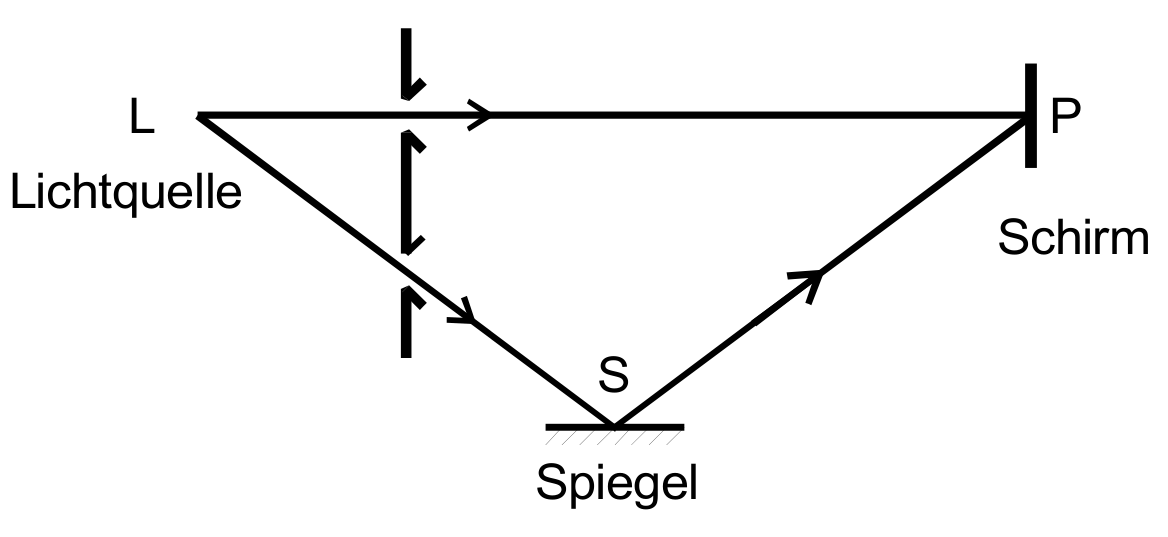
\includegraphics[height=4cm]{ressources/spaltung.png}
  \caption{Aufspaltung und Zusammenführung eines Lichtbündels. \cite{skript}}
  \label{abb:1}
\end{figure}
Beträgt die Differenz der beiden Wege nun ungeradzahlige Vielfache der halben Wellenlänge,
\begin{equation}
  \Delta = (2n+1)\frac{\lambda}{2},
\end{equation}
so kommt es erneut zu Auslöschungseffekten am Punkt P.
Wichtig ist zusätzlich noch die Kohärenzlänge $l$.
Da, wie bereits erwähnt, die Emission von Licht in endlichen Zeitabständen $\tau$ stattfindet, haben die Wellenzüge eine endliche Länge.
Wird diese überschritten, überlagern sich am Zusammentreffungspunkt zwei Wellenzüge von unterschiedlichen Emissionsakten, was bei hinreichend großem Wegunterschied zum Verschwinden des Interferenzeffektes führt.
Demnach wird die Kohärenzlänge festgelegt als das Produkt der bei P maximal beobachtbaren Intensitätsmaxima $N$ mit der Wellenlänge $\lambda$ des Lichtes,
\begin{equation}
  l = N\lambda.\\
\end{equation}
Zusätzlich kann die Breite der Lichtquelle zur Verhinderung der Interferenzerscheinungen führen, da das emittierte Licht an verschiedenen Stellen möglicherweise Phasenverschiebungen aufweist, die in einer insgesamten Inkohärenz enden.\\
Die Quintessenz dieses Abschnittes lautet, dass sich die Wellenlänge einer Lichtquelle über eine Aufspaltung des Lichtes auf verschieden lange Wege, wobei einer um eine Strecke $\Delta l$ variiert wird, und anschließender Zusammenführung der Strahlen durch eine Zählung der entstehenden Interferenzmaxima bestimmen lässt.
Dies genügt der Gleichung
\begin{equation}
  \Delta l = N\frac{\lambda}{2}, \label{eqn:2}
\end{equation}
bei der $N$ die gezählten Interferenzmaxima beschreibt.\\
Dadurch lässt sich auch bei bekannter Wellenlänge die Änderung eines Brechungsindex $\Delta n$,
\begin{equation}
  b\Delta n = N\frac{\lambda}{2}, \label{eqn:3}
\end{equation}
beschreiben, wobei $b$ die Dicke des Probemediums ist.






% 2x2 Plot
% \begin{figure*}
%     \centering
%     \begin{subfigure}[b]{0.475\textwidth}
%         \centering
%         \includegraphics[width=\textwidth]{Abbildungen/Schaltung1.pdf}
%         \caption[]%
%         {{\small Schaltung 1.}}
%         \label{fig:Schaltung1}
%     \end{subfigure}
%     \hfill
%     \begin{subfigure}[b]{0.475\textwidth}
%         \centering
%         \includegraphics[width=\textwidth]{Abbildungen/Schaltung2.pdf}
%         \caption[]%
%         {{\small Schaltung 2.}}
%         \label{fig:Schaltung2}
%     \end{subfigure}
%     \vskip\baselineskip
%     \begin{subfigure}[b]{0.475\textwidth}
%         \centering
%         \includegraphics[width=\textwidth]{Abbildungen/Schaltung4.pdf}    % Zahlen vertauscht ... -.-
%         \caption[]%
%         {{\small Schaltung 3.}}
%         \label{fig:Schaltung3}
%     \end{subfigure}
%     \quad
%     \begin{subfigure}[b]{0.475\textwidth}
%         \centering
%         \includegraphics[width=\textwidth]{Abbildungen/Schaltung3.pdf}
%         \caption[]%
%         {{\small Schaltung 4.}}
%         \label{fig:Schaltung4}
%     \end{subfigure}
%     \caption[]
%     {Ersatzschaltbilder der verschiedenen Teilaufgaben.}
%     \label{fig:Schaltungen}
% \end{figure*}
